%!TEX program = xelatex
\documentclass{standalone}
\usepackage{tikz}

\begin{document}
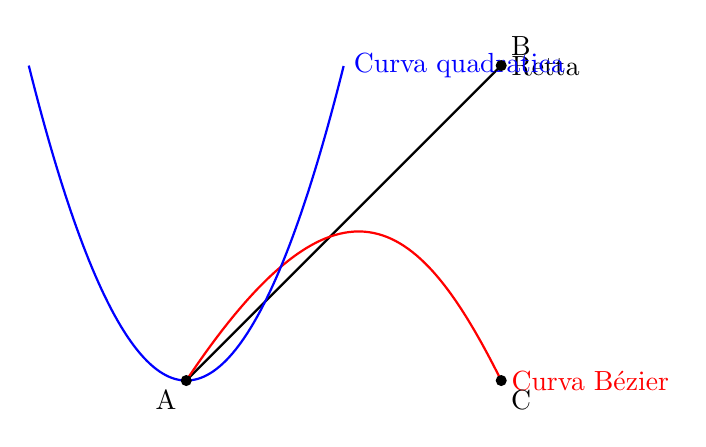
\begin{tikzpicture}

    % Disegna una retta tra due punti
    \draw[thick] (0, 0) -- (4, 4) node[right] {Retta};

    % Disegna una curva di Bézier
    \draw[thick, red] (0, 0) .. controls (2, 3) and (3, 2) .. (4, 0) node[right] {Curva Bézier};

    % Disegna una curva generica con plot
    \draw[blue, thick, domain=-2:2, samples=100] plot (\x, {\x*\x}) node[right] {Curva quadratica};

    % Etichette per i punti
    \fill (0, 0) circle (2pt) node[below left] {A};
    \fill (4, 4) circle (2pt) node[above right] {B};
    \fill (4, 0) circle (2pt) node[below right] {C};

\end{tikzpicture}
\end{document}
